\documentclass[12pt, a4paper, oneside]{ctexart}
\usepackage{amsmath, amsthm, amssymb, bm, graphicx, hyperref, mathrsfs}
\usepackage{tikz}
\usetikzlibrary{arrows.meta, calc, topaths, positioning, automata}

\title{\textbf{Homework}}
\author{PB22010344 黄境}
\date{\today}
\linespread{1.5}
\newcounter{exercisename}
\newenvironment{exercise}{\stepcounter{exercisename}\par\noindent\textsc{Exercise \arabic{exercisename}. }}{\\\par}
\newenvironment{solution}{\par\noindent\textsc{Solution. }}{\\\par}

\DeclareMathOperator{\argmin}{\bf argmin\,}
\DeclareMathOperator{\argmax}{\bf argmax\,}

\begin{document}

\maketitle

\begin{exercise}
    \bf Singular Value Decomposition
\end{exercise}

\begin{solution}
    1. (a)(d) Denote $\mathbf{A}$ by $(\mathbf{a}_1, \mathbf{a}_2, \mathbf{a}_n)^T$. Consider
    \[
    \mathbf{y}_0 = \argmin_{\mathbf{y} \in \mathbb{R}^n} \|\mathbf{x - Ay}\|^2,
    \] 
    we can see that $\mathbf{Ay}_0 = P_{\mathcal{C}(\mathbf{A})}(\mathbf{x})$. Since
    \begin{align*}
    \|\mathbf{x - Ay}\|^2 & = \|\mathbf{x - U}\boldsymbol{\Sigma}\mathbf{V}^T\mathbf{y}\|^2 \\
    & = \|\mathbf{U}^T\mathbf{x} - \boldsymbol{\Sigma}\mathbf{V}^T\mathbf{y}\|^2 \\
    & = \|\mathbf{U}^T\mathbf{x} - \boldsymbol{\Sigma}\mathbf{z}\|^2 \\
    & = \sum_{i=1}^{r}(\mathbf{u}_i^T\mathbf{x} - \sigma_iz_i)^2 + \sum_{i=r+1}^{m}(\mathbf{u}_i^T\mathbf{x})^2
    \end{align*}
    where $\mathbf{z} = \mathbf{V}^T\mathbf{y}$. Therefore, we can set $z_i = \frac{\mathbf{u}_i^T\mathbf{x}}{\sigma_i}$ to fit the equation above, and set $z_{r+1} = \dots = z_m = 0$ to minimize $\|\mathbf{z}\|_2$, leading to
    \[
    \mathbf{y}_0 = \mathbf{Vz} = \mathbf{VSU}^T\mathbf{x},
    \]
    where $\mathbf{S} = diag(\sigma_1^{-1}, \sigma_2^{-1}, \dots, \sigma_r^{-1}, 0, \dots, 0)$. Thus, we have
    \[
    P_{\mathcal{C}(\mathbf{A})}(\mathbf{x}) = \mathbf{U}\boldsymbol{\Sigma}\mathbf{V}^T\mathbf{VSU}^T\mathbf{x} = \mathbf{U}\boldsymbol{\Sigma}\mathbf{SU}^T\mathbf{x} = \mathbf{U}diag(\mathbf{I}_r, 0)\mathbf{U}^T = \mathbf{U}_1\mathbf{U}_1^T\mathbf{x}.
    \]
	Next, we will prove (d) in three steps. Since
	\[
	\mathbf{a}_i^T\mathbf{y} = 0,\, \forall\, \mathbf{y} \in \mathcal{N}(\mathbf{A}^T), 
	\]
	and
	\[
	\mathbf{z} = \sum_{i=1}^{n}\lambda_i\mathbf{a}_i,\, \forall\, \mathbf{z} \in \mathcal{C}(\mathbf{A}),
	\]
	we have
	\[
	\mathbf{z}^T\mathbf{y} = \sum_{i=1}^{n}\lambda_i\mathbf{a}_i^T\mathbf{y} = 0,\, \forall\, \mathbf{y} \in \mathcal{N}(\mathbf{A}^T), \mathbf{z} \in \mathcal{C}(\mathbf{A}),
	\]
	that is, $\mathcal{C}(\mathbf{A}) \bot \mathcal{N}(\mathbf{A}^T)$. \newline
	Since $\mathcal{C}(\mathbf{A})$ and $\mathcal{N}(\mathbf{A}^T)$ are closed linear subspaces in $\mathbb{R}^m$, by the orthogonal decomposition we have learned in functional analysis class, we have
	\[
	\forall \mathbf{x} \in \mathbb{R}^m,\, \exists\, \mathbf{y} \in \mathcal{C}(\mathbf{A}), \mathbf{z} \in \mathcal{N}(\mathbf{A}^T), \text{ s.t. } \mathbf{x = y + z}.
	\]
	Moreover, $\mathbf{y}$ is the element of best approximation of $\mathbf{x}$ on the subspace $\mathcal{C}(\mathbf{A})$, which is exactly $P_{\mathcal{C}(\mathbf{A})}(\mathbf{x})$. Therefore, $\mathbf{z} = \mathbf{x - y}$ satisfies
	\[
	\mathbf{x - z} = \mathbf{x - x + y} = \mathbf{y} = P_{\mathcal{C}(\mathbf{A})}(\mathbf{x}) \in \mathcal{C}(\mathbf{A}) \quad \Rightarrow \quad \mathbf{x - z} \bot \mathcal{N}(\mathbf{A}^T)
	\]
	which is the best approximation condition. Thus, $\mathbf{z}$ is the element of best approximation of $\mathbf{x}$ on the subspace $\mathcal{N}(\mathbf{A}^T)$, which implies that
	\[
	\mathbf{z} = P_{\mathcal{N}(\mathbf{A}^T)}(\mathbf{x}) = \mathbf{x - y} = \mathbf{x} - \mathbf{U}_1\mathbf{U}_1^T\mathbf{x} = (\mathbf{I} - \mathbf{U}_1\mathbf{U}_1^T)\mathbf{x} = \mathbf{U}_2\mathbf{U}_2^T\mathbf{x},
	\]
	thus complete the proof.
	\newline\newline
	(b)(c) Since $\mathbf{A}^T = \mathbf{V}\boldsymbol{\Sigma}^T\mathbf{U}^T = \mathbf{V}\boldsymbol{\Sigma}\mathbf{U}^T$, we can obtain these conclusions by following the same steps in (a)(d).
	\newline\newline
    2.(a) Since
    \[
    (\mathbf{A}^T\mathbf{A})_{ii} = \sum_{j=1}^{m}a_{ji}\cdot a_{ji} = \sum_{j=1}^{m}a_{ji}^2,
    \]
    we have
    \[
    tr(\mathbf{A}^T\mathbf{A}) = \sum_{i=1}^{n}(\mathbf{A}^T\mathbf{A})_{ii} = \sum_{i=1}^{n}\sum_{j=1}^{m}a_{ji}^2 = \|\mathbf{A}\|_F^2
    \]
    \newline
    (b) Let $\mathbf{a} = \mathbf{Ae}_i$, $\mathbf{b} = \mathbf{Be}_i$, $i\in[n]$, we have
    \[
    \langle\mathbf{a},\mathbf{b}\rangle = \mathbf{e}_i^T\mathbf{A}^T\mathbf{Be}_i = (\mathbf{A}^T\mathbf{B})_{ii} = \sum_{j=1}^{m}a_{ji}b_{ji} = 0.
    \]
    which implies that
    \[
    tr(\mathbf{A}^T\mathbf{B}) = \sum_{i=1}^{n}\sum_{j=1}^{m}a_{ji}b_{ji} = 0.
    \]
    Therefore, we have
    \begin{align*}
    \|\mathbf{A+B}\|_F^2 & = \sum_{i=1}^{m}\sum_{j=1}^{n}(a_{ij}+b_{ij})^2 \\
    & = \|\mathbf{A}\|_F^2 + \|\mathbf{B}\|_F^2 + 2\sum_{i=1}^{m}\sum_{j=1}^{n}a_{ij}b_{ij} \\
    & = \|\mathbf{A}\|_F^2 + \|\mathbf{B}\|_F^2 + 2tr(\mathbf{A}^T\mathbf{B}) \\
    & = \|\mathbf{A}\|_F^2 + \|\mathbf{B}\|_F^2
    \end{align*}
\end{solution}

\begin{exercise}
	\bf Principle Component Analysis
\end{exercise}

\begin{solution}
	1. We have
	\begin{align*}
	f(\mathbf{GQ}) = tr((\mathbf{GQ})^T\mathbf{SCQ}) & = tr(\mathbf{Q}^T\mathbf{G}^T\mathbf{SGQ}) \\
	& = tr(\mathbf{QQ}^T\mathbf{G}^T\mathbf{SG}) \\
	& = tr(\mathbf{G}^T\mathbf{SG}) = f(\mathbf{G})
	\end{align*}
	\newline
	2. Since $\mathbf{g}_1^T\mathbf{Sg}_1 \in \mathbb{R}$, we have $f(\mathbf{g}) = \mathbf{g}_1^T\mathbf{Sg}_1$. Therefore, the Lagrange function is
	\[
	L(\mathbf{g},\lambda) = f(\mathbf{g}) + \lambda(1 - \|\mathbf{g}\|^2_2).
	\]
	Since $\mathbf{S}$ is symmetric, taking derivative and we get
	\[
	\mathbf{Sg} + \mathbf{Sg} - 2\lambda\mathbf{g} = 0 \quad \Rightarrow \quad \mathbf{Sg} = \lambda\mathbf{g},
	\]
	which implies that $\mathbf{g}$ is an eigenvector of $\lambda$. Suppose that $\boldsymbol{\Lambda} = \{\lambda_1$, $\lambda_2$, ..., $\lambda_r\}$ are all if the eigenvalues of $\mathbf{S}$, where $\lambda_1 \geq \lambda_2 \geq \dots \geq \lambda_r$. Let $\mathbf{G} = \{\mathbf{g}_1$, $\mathbf{g}_2$, ..., $\mathbf{g}_r\}$ are corresponding eigenvectors with length $1$, we have
	\[
	\argmax_{\mathbf{g}_i \in \mathbf{G}}\{\mathbf{g}_i^T\mathbf{Sg}_i\} = \argmax_{\mathbf{g}_i \in \mathbf{G}}\{\lambda_i\mathbf{g}_i^T\mathbf{g}_i\} = \argmax_{\mathbf{g}_i \in \mathbf{G}}\{\lambda_i\} = \mathbf{g}_1. 
	\]
	which is the first principal component vector of the data.
	\newline\newline
	3. The Lagrange function is
	\[
	L(\mathbf{g}, \lambda, \mu) = f(\mathbf{g}) + \lambda(1 - \|\mathbf{g}\|^2_2) - \mu\langle\mathbf{g}, \mathbf{g}_1\rangle.
	\]
	Taking derivative and we get
	\begin{align*}
	& 2\mathbf{Sg} - 2\lambda\mathbf{g} - \mu\mathbf{g}_1 = 0 \\
	& \Rightarrow 2\mathbf{g}_1^T\mathbf{Sg} - 2\lambda\mathbf{g}_1^T\mathbf{g} - \mu\mathbf{g}_1^T\mathbf{g}_1 = 0 \\
	& \Rightarrow \mu = 2\mathbf{g}_1^T\mathbf{Sg} - 2\lambda\mathbf{g}_1^T\mathbf{g} = 2\lambda_1\mathbf{g}_1^T\mathbf{g} = 0
	\end{align*}
	Therefore, we have
	\[
	\mathbf{g}_2 = \argmax_{\mathbf{g}_i \in \mathbf{G}, \mathbf{g}_i \neq \mathbf{g}_1}\{\lambda_i\} = \lambda_2.
	\]
	is the second principal component vector of the data.
	\newline\newline
	4. From the same steps, we have
	\[
	\mathbf{g}_K = \argmax\{f(\mathbf{g}):\|\mathbf{g}\| = 1,\langle\mathbf{g}_i, \mathbf{g}\rangle = 0, i = 1, 2, \dots, K-1\}
	\]
	\newline
	5. From the content in exercise 10.1 in HW1, we know that $f(\mathbf{g}_K) = \lambda_K$, which is the K-th largest eigenvalue of $\mathbf{S}$.
\end{solution}

\begin{exercise}
	\bf Properties of Transition Matrix
\end{exercise}

\begin{solution}
	1. Set $\mathbf{a} = (1, 1, \dots, 1)^T$, we have
	\[
	\mathbf{Ta} = (\sum_{i=1}^{n}t_1i, \sum_{i=1}^{n}t_2i, \dots, \sum_{i=1}^{n}t_ni)^T = (1, 1, \dots, 1)^T,
	\]
	which implies that $1$ is a eigenvalue of $\mathbf{T}$.
	\newline\newline
	2. From exercise 10.1 in HW1, we can estimate $\sup\limits_{\|\mathbf{x}\|=1}\mathbf{x}^T\mathbf{Tx} = \lambda_{max}$ directly.
	\begin{align*}
	\sup\limits_{\|\mathbf{x}\|=1}\mathbf{x}^T\mathbf{Tx} & = \sup\limits_{\sum_{i=1}^{n}x_i^2 = 1}\sum_{i,j=1}^{n}x_ix_jt_{ij} \\
	& = \sup\limits_{\sum_{i=1}^{n}x_i^2=1}\sum_{i,j=1}^{n}x_i\sqrt{t_{ij}}x_j\sqrt{t_{ij}} \\
	& \leq \frac{1}{2}\sup\limits_{\sum_{i=1}^{n}x_i^2=1} \sum_{i,j=1}^{n}x_i^2t_{ij} + x_j^2t_{ij} \\
	& = \frac{1}{2}\sup\limits_{\sum_{i=1}^{n}x_i^2=1} (\sum_{i=1}^{n}x_i^2(\sum_{j=1}^{n}t_{ij})) + (\sum_{j=1}^{n}x_j^2(\sum_{i=1}^{n}t_{ij})) \\
	& = \frac{1}{2}\sup\limits_{\sum_{i=1}^{n}x_i^2=1}\sum_{i=1}^{n}x_i^2 + \sum_{j=1}^{n}x_j^2 \\
	& = \sup\limits_{\sum_{i=1}^{n}x_i^2=1}\sum_{i=1}^{n}x_i^2 = 1
	\end{align*}
	Therefore, $\lambda_{max} \leq 1$. On the other hand, 
	\begin{align*}
	\lambda_{min} & = \inf\limits_{\|\mathbf{x}\|=1}\mathbf{x}^T\mathbf{Tx} \\
	& = \inf\limits_{\sum_{i=1}^{n}x_i^2=1}\sum_{i,j=1}^{n}x_i\sqrt{t_{ij}}x_j\sqrt{t_{ij}} \\
	& \geq \frac{1}{2} \inf\limits_{\sum_{i=1}^{n}x_i^2=1}\sum_{i,j=1}^{n}-x_i^2t_{ij} - x_j^2t_{ij} \\
	& = -1
	\end{align*}
	Combining together, we have $|\lambda| \leq 1$.
	\newline\newline
	3. From the discussion below, we have 
	\[
	\inf\limits_{\|\mathbf{x}\|=1}\mathbf{x}^T(\mathbf{I} - \gamma\mathbf{T})\mathbf{x} = 1 - \gamma\sup\limits_{\|\mathbf{x}\|=1}\mathbf{x}^T\mathbf{Tx} \geq 1 - \gamma > 0.
	\]
	Since $\mathbf{x}^T(\mathbf{I} - \gamma\mathbf{T})\mathbf{x} = \frac{\mathbf{x}^T}{\|\mathbf{x}\|}(\mathbf{I} - \gamma\mathbf{T})\frac{\mathbf{x}}{\|\mathbf{x}\|} \cdot \|\mathbf{x}\|^2$, we have
	\[
	\mathbf{x}^T(\mathbf{I} - \gamma\mathbf{T})\mathbf{x} \geq \|\mathbf{x}\|^2 \inf\limits_{\|\mathbf{x}\|=1}\mathbf{x}^T(\mathbf{I} - \gamma\mathbf{T})\mathbf{x} \geq \|\mathbf{x}\|^2 (1 - \gamma) > 0,
	\]
	for all $\mathbf{x} \in \mathbb{R}^n$ and $\|\mathbf{x}\| \neq 0$, which implies that $\mathbf{I} - \gamma\mathbf{T} \succ 0$, thus $\mathbf{I} - \gamma\mathbf{T}$ is invertible.
\end{solution}

\begin{exercise}
	\bf Planning with a Two-Armed Bandit
\end{exercise}

\begin{solution}
	1. We have
	\[
	\mathbf{\mathcal{S}} = \{state\_1, state\_2\} = \{s_1, s_2\},
	\]
	and
	\[
	\mathbf{\mathcal{A}} = \{pull\_bandit\_1, pull\_bandit\_2\} = \{a_1, a_2\}.
	\]
	Therefore,
	\begin{align*}
	& P(s_1|s_1,a_1) = 1, && P(s_2|s_1,a_1) = 0. \\
	& P(s_1|s_1,a_2) = 0.6, && P(s_2|s_1,a_2) = 0.4. \\
	& P(s_1|s_2,a_1) = 0, && P(s_2|s_2,a_1) = 1. \\
	& P(s_1|s_2,a_2) = 0.8, && P(s_2|s_2,a_2) = 0.2.
	\end{align*}
	Markov process diagram:\newline
	\begin{center}
		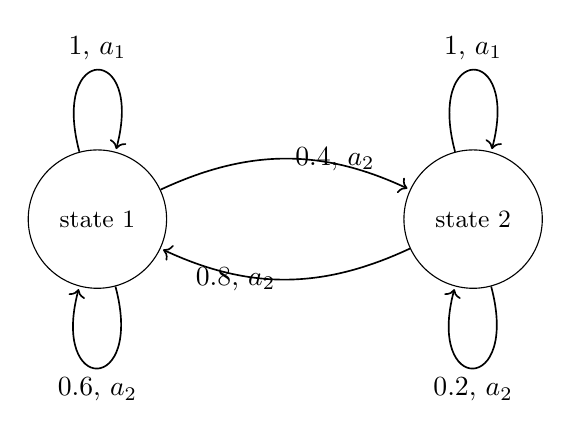
\begin{tikzpicture}[node distance=3cm,
		                    every state/.style={align=center, node font=\small, minimum size=50pt}]
		  \node[state] (s1)                             {state 1};
		  \node[state] (s2) [right=of s1]               {state 2};
		  
		  \path[->, bend angle=25, shorten >=1pt, semithick] 
		  	(s1)	edge[loop above]	node		{1, $a_1$}		()
		  			edge[loop below]	node		{0.6, $a_2$}	()
		  			edge[bend left]		node[right]	{0.4, $a_2$}	(s2)
		  	(s2)	edge[loop above]	node		{1, $a_1$}		()
		  			edge[loop below]	node		{0.2, $a_2$}	()
		  			edge[bend left]		node[left]	{0.8, $a_2$}	(s1);
		\end{tikzpicture}
	\end{center}
	2.(a) We have
	\begin{align*}
	V^{\pi_1}(s_1) & = \mathbb{E}[r(s_1, a_2)] + \gamma\mathbb{E}[G_{t+1}] \\
	& = 0 + \gamma(P(s'=s_1)V^{\pi_1}(s_1) + P(s'=s_2)V^{\pi_1}(s_2)) \\
	& = 0.54 V^{\pi_1}(s_1) + 0.36 V^{\pi_1}(s_2)
	\end{align*}
	and
	\begin{align*}
	V^{\pi_1}(s_2) & = \mathbb{E}[r(s_2, a_2)] + \gamma\mathbb{E}[G_{t+1}] \\
		& = 3 + \gamma(P(s'=s_1)V^{\pi_1}(s_1) + P(s'=s_2)V^{\pi_1}(s_2)) \\
		& = 3 + 0.72 V^{\pi_1}(s_1) + 0.18 V^{\pi_1}(s_2)
	\end{align*}
	Combining together, we have
	\[
	V^{\pi_1}(s_1) = 9.1525,\, \quad V^{\pi_1}(s_2) = 11.6949.
	\]
	\newline
	(b) Similarly,
	\begin{align*}
	V^{\pi_2}(s_1) & = \mathbb{E}[r(s_1, a_2)] + \gamma\mathbb{E}[G_{t+1}] \\
	& = 0 + \gamma(P(s'=s_1)V^{\pi_2}(s_1) + P(s'=s_2)V^{\pi_2}(s_2)) \\
	& = 0.54 V^{\pi_2}(s_1) + 0.36 V^{\pi_2}(s_2)
	\end{align*}
	\begin{align*}
	V^{\pi_2}(s_2) & = \mathbb{E}[r(s_2, a_1)] + \gamma\mathbb{E}[G_{t+1}] \\
		& = 2 + \gamma(P(s'=s_1)V^{\pi_2}(s_1) + P(s'=s_2)V^{\pi_2}(s_2)) \\
		& = 2 + 0.9 V^{\pi_2}(s_2)
	\end{align*}
	We have
	\[
	V^{\pi_1}(s_1) = 15.6522,\, \quad V^{\pi_1}(s_2) = 20.
	\]
	\newline
	3. We have these policies:
	\begin{align*}
	& \pi_1: \pi_1(s_1) = a_1, \pi_1(s_2) = a_1. \\
	& \pi_2: \pi_1(s_1) = a_2, \pi_1(s_2) = a_2. \\
	& \pi_3: \pi_1(s_1) = a_1, \pi_1(s_2) = a_2. \\
	& \pi_4: \pi_1(s_1) = a_2, \pi_1(s_2) = a_1. \\
	\end{align*}
	Since $V = (\mathbf{I} - \gamma\mathbf{T})^{-1}\mathbf{R}$, we have
	\[
	\mathbf{T}_1 = 
		\begin{pmatrix}
		1 & 0 \\
		0 & 1 \\
		\end{pmatrix},
	\mathbf{T}_2 = 
		\begin{pmatrix}
		0.6 & 0.4 \\
		0.8 & 0.2 \\
		\end{pmatrix},
	\mathbf{T}_3 = 
		\begin{pmatrix}
		1 & 0 \\
		0.8 & 0.2 \\
		\end{pmatrix},
	\mathbf{T}_4 = 
		\begin{pmatrix}
		0.6 & 0.4 \\
		0 & 1 \\
		\end{pmatrix}.
	\]
	and
	\[
	\mathbf{R}_1 = (1, 2)^T,
	\mathbf{R}_2 = (0, 3)^T,
	\mathbf{R}_3 = (1, 3)^T,
	\mathbf{R}_4 = (0, 2)^T.
	\]
	For $\gamma = 0.1$,
	\[
	V_1 = (1.11, 2.22)^T,
	V_2 = (0.13, 3.07)^T,
	V_3 = (1.11, 3.15)^T,
	V_4 = (0.10, 2.22)^T,
	\]
	and we can see that the best policy here is $\pi_3$. \newline
	For $\gamma = 0.99$, similarly we get
	\[
	V_1 = (100, 200)^T,
	V_2 = (99.17, 101.67)^T,
	V_3 = (100, 102.49)^T,
	V_4 = (195.07, 200)^T,
	\]
	which means we have the best policy $\pi_4$ here. \newline
	$\gamma$ can be understood as the discount rate in finance, which represents the ratio of expected returns in a certain period of time in the future to present value based on the time value of money. High $\gamma$ value mean a greater focus on future earnings, while low $\gamma$ value aims to get more profits in short term.
\end{solution}

\end{document}